\documentclass{article}
\usepackage[utf8]{inputenc}
\usepackage[english]{babel}
\usepackage{amsthm}
\usepackage{amssymb}
\usepackage{mathtools}
\usepackage{enumerate}
\newcommand\tab[1][1cm]{\hspace*{#1}}
\usepackage{graphicx}

\author{Kevin Martin\\ CIS675 - Syracuse University}
\title{Homework 3}

\newtheorem*{claim}{Question}
\renewcommand\qedsymbol{$\blacksquare$} 
\begin{document}
\maketitle
\begin{enumerate}
    \item Question 3
      \begin{enumerate}
    \item \ Pseudocode for a greedy algorithm to compute optimal order and minimize wait time:\\\\
      Sort the service time in ascending order, and serve them in order of increasing scheduling
            times. \\
            Let n be the list of customers that need to be solved, with each time required $t_{i}$
            as the relevent index in the array:\\
      
      def greedySort(n [])\\
      sort(n); // in ascending order\\
      currentJob = n[1]\\
      for i = 1 to n:\\
          \tab currentJob = currentJob + $t_{i}$

             
    \item Claim: the running time of the proposed algorithm is $O(n logn)$
      \begin{proof}
      Sorting the list to get the algorithm started is where most of the time is required. Sorting a
        list of $n$ elements takes $O(nlogn)$ time. The rest of the algorithm can be completed in constant
        time, $O(1)$. Because the algorithm can be written as $c_{1}+(c_{1}+c_{2})+(c_{1}+c_{2}+...c_{n})
        \frac 1 n$, we can see that $c_{1}$ repeats itself the most times. As such, because it is the shortest
        time, then no other ordering could be correct. Therefore the greedy strategy holds true.

      \end{proof}

  \end{enumerate}
    \item Question 5
      \begin{enumerate}
        \item To represent the situation as a linear problem, we formulate as follows, letting 
          $x_{1}$ be coffee mugs and $x_{2}$ be milk glasses:\\
          \tab Objective function \tab max $25x_{1}+20x_{2}$  \\
          \tab Constraints \tab \tab $20x_{1}+12x_{2} \leq 1800$  \\
          \tab \tab \tab \tab \tab $x_{1}/15+x_{2}/15 \leq 8$\\
          \tab \tab \tab \tab \tab $x_{1},x_{2} \geq 0$\\


        \item Graph of feasible region:



        \item The coordinates of all vertices of the feasible region are:\\
          (0, 0), (90, 0), (45, 75), (0, 120)

        \item The optimal product mix to maximize daily proift is:\\
          45 coffee mugs at \$ 25 each and 90 milk glasses at \$ 20 each 
          gives a total profit of \$2,625 per day.
          This is represented on the graph but the furthest out point on on the 
          feasible region, represented by the tangential dotted line.




      \end{enumerate}

\item Question 3\\\\
  \begin{enumerate}
  \item The adjacency matrix representation:\\
  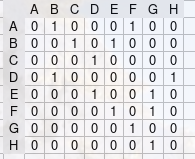
\includegraphics[scale=1]{adjmatrix.png}
  
  \item The adjacency list representation:\\
    $A: B \to F$\\
    $B: C \to E$\\
    $C: D$\\
    $D: B \to H$\\
    $E: D \to G$\\
    $F: E \to G$\\
    $G: F$\\
    $H: G$
    
    \item Table for intermediate visited, pre, and post values of all nodes:\\
    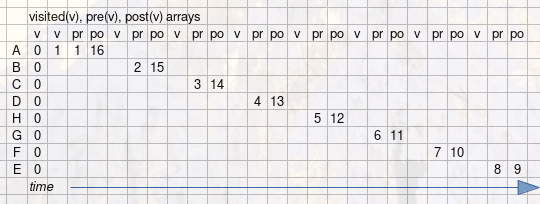
\includegraphics[width=\textwidth]{inttable.png}\\
    \pagebreak
    \item Final DFS tree:\\
    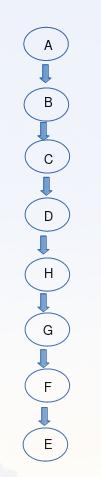
\includegraphics[scale=1]{dfstree.png}


  \end{enumerate}
\pagebreak
\item Question 4\\\\
  Pseudocode of an efficient algorithm to take in graph G(V, E), represetned by an adjacency list,
    and two vertices $x, y \in V$, where the output is the different paths from $x$ to $y$ in G:\\\\
    //wrapper function to set empty path\\
    def diffPathsWrap(x, y, G)\\
    for i = 1 to (size-1) do\\
    \tab visited[i] = False\\     
    \tab path = [] //empty array for each path\\
    diffPaths(x, y, G, path)\\\\

    def diffPaths(x,y, visited, path)\\
    visited[x]=True\\
    if x == y\\
    \tab return path\\
    else\\
    \tab for j in G[x] do\\
    \tab \tab if visited[j] == False\\
    \tab \tab \tab return diffPaths(x, y, visited, path)\\
   \tab \tab path[j].remove //remove current vertex from path\\
   \tab \tab visited[j] = False

\item Question 5\\
  \begin{enumerate}
      \item The order of the strongly connected componets is:\\
        $A \to B \to E$\\
        $C$\\
        $D \to H \to F \to I \to H \to D$
      \item The source SCC is $A \to B \to E$ and the sink SCC 
        is $D \to H \to F \to I \to H \to D$\\
        \pagebreak
      \item Metagraph:\\
      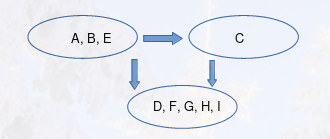
\includegraphics[width=\textwidth]{metagraph.png}
      \item The minimum number of edges one must add to make the graph 
        strongly connected is just one: from $D \to G$. If that edge were
        added, then we could get to any vertex from any other.


  \end{enumerate}
\end{enumerate}
\end{document}


